\chapter{Selective DNA sequencing}
% TODO, vysvetlit eventy
\label{kap:selSeq}

In this chapter, we explain the term selective sequencing. We highlight the
advantages of this method and look at the current state of research in this area.

\section{DNA}

% TODO: pridat zdroj %https://en.wikipedia.org/wiki/Genetics#DNA_sequencing_and_genomics
Genetics is a branch of biology that studies genes, genetic variation, and heredity.
It tries to explain the variability between animals, the source of hereditary diseases, and
other important things that influence our lives. The DNA is the key molecule
that stores biological information in living organisms. It is contained in
almost every living cell. Based on the information from this molecule, our cells can reproduce and create copies of
themselves. Nowadays, it is possible to look at the DNA of the organism. This ability is
one of the strongest tools of genetics as it helps us tell what are the functions
of different parts of DNA by comparing it between organisms and looking at the
consequences of different mutations.

DNA stores genetic information in the form of a sequence of nucleotides. Their particular order defines the stored
information. There are four types of DNA nucleotides:
adenine (A), cytosine (C), guanine (G) and thymine (T). DNA consists of two long
strings of these nucleotides that together create the DNA molecule. The two strands
are connected in a complementary way. If there is A on the forward strand,
then there is T on the reverse. If there is a C on the one strand, we can expect
it's complement G on the other one. In this way, the cell machinery can (to some extent) repair
missing nucleotides based on the complement rules. An example of how we can think
of DNA is on \ref{obr:acgt}.

From now, we will represent the DNA sequence as a sequence of characters A, C, G, T.
Such representation stores enough information so we can recover the other complementary
DNA strand easily.

% TODO: obrazok zdroj https://www.genome.gov/genetics-glossary/acgt

\begin{figure}
\centerline{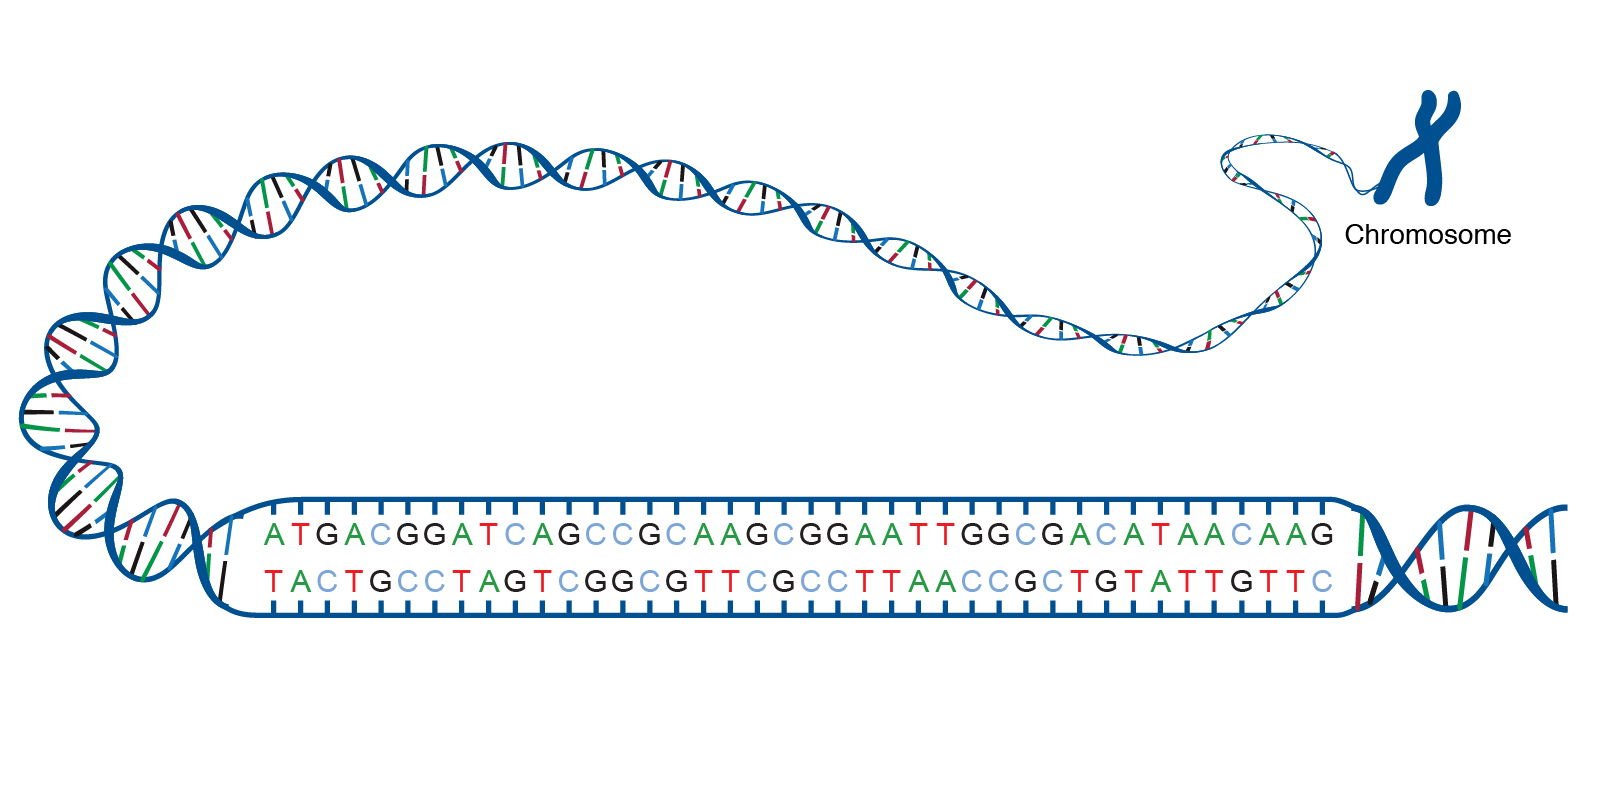
\includegraphics[width=0.7\textwidth, height=0.3\textheight]{images/acgt}}
\caption[DNA]{DNA Molecule}
\label{obr:acgt}
\end{figure}

\section{DNA sequencing}

The process of obtaining DNA sequence is called \textit{DNA sequencing}.
The DNA molecule is very long, and processing it whole at once would be very hard.
Single DNA molecule in one cell can reach up to 2 meters when untangled.
%https://www.sciencefocus.com/the-human-body/how-long-is-your-dna/
Thus, it is convenient to broke down the whole DNA molecule into many shorter fragments.
This can be done chemically. Once we have this mixture of shorter DNA molecules, we need to sequence individual
shorter fragments and then somehow connect them to obtain the nucleotide string representing
our original DNA molecule. One of the devices that can sequence the mixture of the
DNA fragmentsMinION\cite{lu2016oxford}. MinION is a cheap and versatile DNA sequencer
with the size of the larger USB key (see in Figure \ref{obr:minIon}).

\begin{figure}
\centerline{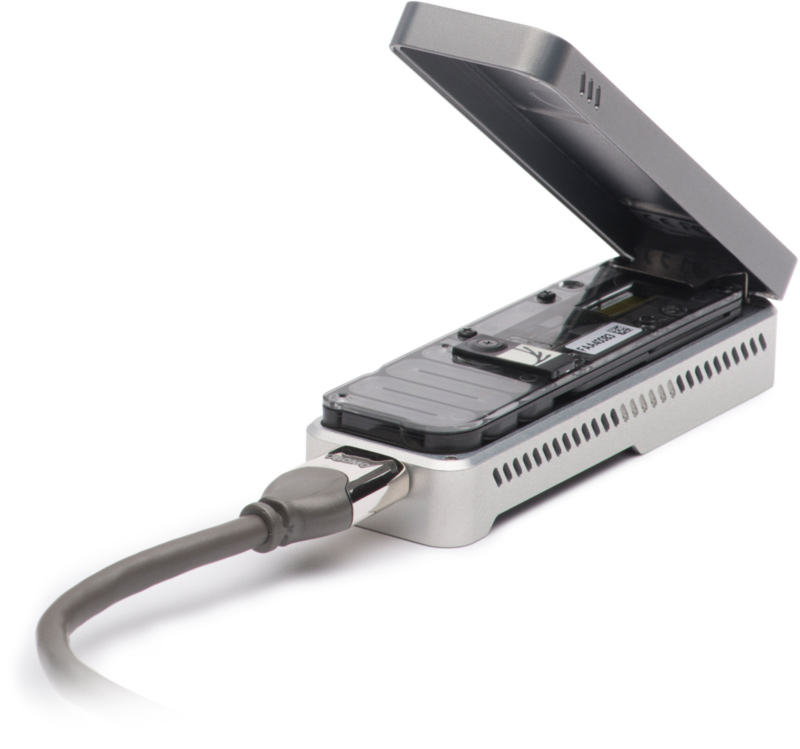
\includegraphics[width=0.7\textwidth, height=0.3\textheight]{images/minion}}
\caption[MinION]{MinION sequencer}
\label{obr:minIon}
\end{figure}

MinION consists of an active surface filled with many \textit{nanopores}. A nanopore
is a small hole with an electric current passing through it. When the positive charge
is generated on the other side of the surface, negatively charged DNA molecules
will start to pass through the pores. As the molecule of DNA is passing through the pore of
MinION, we can observe changes in the flow of an electric current passing through the pore.
This electric current is measured over the discrete-time and it is called \textit{signal},
\textit{raw signal} or \textit{squiggle}. The example of the squiggle is shown in Figure \ref{obr:minIonCurrent}.

\begin{figure}
\centerline{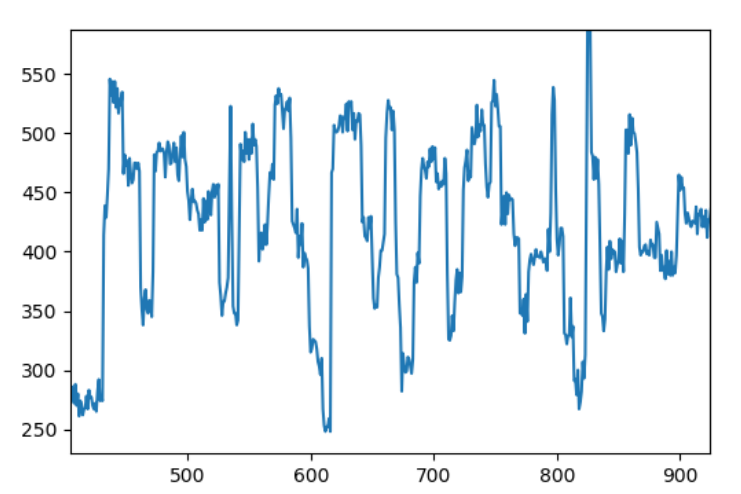
\includegraphics[width=0.7\textwidth, height=0.3\textheight]{images/signal}}
\caption[MinION signal]{Electric current (squiggle) coming from MinION.}
\label{obr:minIonCurrent}
\end{figure}

Currently, MinION processes around 450 nucleotides per second for each nanopore.
The value of the current signal is measured 4000 times per second so each
nucleotide produces on average about 8-9 \textit{readouts}. The signal
generated from the pass of the single DNA molecule through the single pore is called \textit{read}.
One of the advantages of the MinION sequencer is that it produces very long reads.
The length of the read is stated in kb(kilo-bases) where base corresponds to one nucleotide.
The mean length of the read in some scenarios ranges from 13kb to 20kb. Additionally,
since MinION has 200-500 nanopores, it can produce large amounts of
data very quickly.

% TODO: https://www.ncbi.nlm.nih.gov/pmc/articles/PMC5793790/

After obtaining the raw signal from the pore, it needs to be finally converted into the DNA
sequence. Importantly, as the DNA passes through the pore, only a small
number of nucleotides in the proximity of the pore influence the current output signal.

The output signal of MinION is mostly dependent only on the context of the k
nucleotides(also called \textit{k-mers} present in the proximity of the pore. There are several studies on
how much is signal influenced by more distant nucleotides. It is generally accepted
that using the $k = 6$ is appropriate for building an accurate model of the signal. 
Usually, with the MinION, we are provided with a kmer model.

In general, the signal model is a list of all possible $k$-mers for some $k$
that states the mean and standard deviation of a Gaussian distribution that
describes expected distribution signal readout for that particular $k$-mer.
Using the measurements of signal over time, using a method called base-calling, we can reconstruct the
the sequence of the DNA molecule that produced that signal.

Early base-calling algorithms tried to split the signal into \textit{events}\cite{david2017nanocall}.
Event is a longer sequence of signals at the roughly same level corresponding
to one particular $k$-mer. Using a k-mer model on events, as well as information
that k-mers following each should overlap, one can predict the sequence that passed through this pore.

Nowadays, more successful base-calling algorithms are based on recurrent neural
networks. Despite significant improvements in the base-calling algorithms, the overall
process of base-calling is quite slow and resource-intensive.

After the base-calling, we need to join this all base-called reads together to form the
resulting DNA sequence. This is quite hard as the base-calling process is not entirely
accurate and produces some errors. Thanks to the duplication of the shorter DNA
sequences, we are, in most cases able to reconstruct the original DNA string.

\section{Selective sequencing}

MinION has an ability to reject DNA molecule that is currently passing through
the pore. MinION reverses the molecule's direction and throws it away.
\textit{Selective sequencing} is the idea that based on the incoming signal, one can determine
whether we are interested in sequencing the current DNA molecule. Subsequently, we can decide if we want
to continue or reject this molecule. This happens on-the-fly, so we need to make
the decision as quickly as possible for the process to be effective.

There are many benefits of selective sequencing. In case we are not interested
in some DNA that we know is contained in our sample, we can use this technique to
reject unwanted DNA molecules. This saves us a lot of time and resources as obtaining
nucleotide sequence from the signal is in some scenarios unnecessary and too
costly process in terms of performance.

For example, consider a scenario when attempting to sequence a pathogen (bacteria, virus) in human blood. We can
reject all human DNA molecules because we are not interested in sequencing human
DNA. We could also filter positively. So we could say that we are only
interested in sequencing DNA that produces a signal in some sense similar to our
chosen sample. This all means saving a lot of resources, for example during the disease diagnosis process.

Naturally, there are some drawbacks to selective sequencing. In order to find out
if the currently passing molecule is from human DNA, we have to have some information
about the signal from human DNA beforehand. This is limiting as we need a sample signal from
the species that we want to filter. The other problem is that in the case of misclassifying
some signal as not interesting, we lose information about the corresponding
part of the DNA molecule.

The idea of accessing real-time data during the phase of reading the DNA molecules
and rejecting the DNA molecule based on this data is called \textit{Read Until}. 

\section{Current state of selective sequencing}
\label{section:currState}

%https://www.nature.com/articles/nmeth.3930
%https://www.biorxiv.org/content/10.1101/038760v1

One approach to selective sequencing is to base-call the current read
and try to match it in the reference sequence. If we could not match this read
into any part of the reference, we can discard the DNA molecule.

The base-calling process, however, is quite slow and our decision must be done on-the-fly.
This often means we do not have time to turn our signal into a nucleotide sequence
as the reads are too short for this and can be already sequenced when we made our decision.

In this thesis, we will work directly with the raw signal to ascertain whether the molecule
should be sequenced or not. One approach (see \cite{loose2016real}) is to obtain the reference signal using
simulation from the reference nucleotide string. We then use an algorithm called
the dynamic time warping (DTW) to align the signal from the read to this reference signal.
The DTW is a dynamic programming algorithm that takes two signals and aligns them in a
way that minimizes the total number of insertions and deletions. One of the limitations
of DTW is that it has run time complexity $\mathcal{O}(n\cdot m)$ where $n$ and $m$
is the length of the reference signal and read respectively. This would pose a problem
for this method if we wanted to use it for longer sequences.

Another useful tool that we will heavily use during the testing of our method is
nanopore data variant caller (Nadavca). It is a convenient tool that requires a reference
DNA sequence and squiggle. Nadavca can create the simulated reference signal
and search for our squiggle in this signal using the already mentioned DTW algorithm.
One drawback is that it is not fast enough to be used for selective sequencing.

In our work, we attempt to improve the results of the work with the squiggles.
We focus on the scenario, where we are given a reference sequence of the DNA. We
will attempt to distinguish between the signal originating from this DNA and the
signal unrelated to the reference.
